% Three stages of XGBoost's history; the waffle shows 17 of the 29 winning Kaggle solutions of 2015 (Chen and Guestrin 2016, 1).
\documentclass[tikz,border=8pt]{standalone}
% Shared look for every TikZ diagram. Load with \input{../../tools/tikz-style.tex}
\usepackage[T1]{fontenc}
\usepackage{lmodern}
\renewcommand{\sfdefault}{lmr}  % diagrams use the same serif as the text
\usetikzlibrary{arrows.meta, positioning, shapes.geometric, calc, fit, backgrounds}
\definecolor{cblue}{HTML}{4C78A8}
\definecolor{corange}{HTML}{F58518}
\definecolor{cgreen}{HTML}{54A24B}
\definecolor{cred}{HTML}{E45756}
\definecolor{cpurple}{HTML}{B279A2}
\definecolor{cgrey}{HTML}{6B6B6B}
\tikzset{
  every picture/.style={font=\sffamily, line width=1.2pt},
  box/.style={draw=#1, fill=#1!12, rounded corners=4pt, align=center, inner sep=7pt, minimum height=1.1cm},
  box/.default=cgrey,
  arrow/.style={-{Stealth[length=3mm]}, draw=cgrey, line width=1.4pt},
  title/.style={font=\sffamily\bfseries\Large},
  note/.style={font=\sffamily\small, text=cgrey, align=center},
}
\AtBeginDocument{\hyphenpenalty=10000 \exhyphenpenalty=10000}

\begin{document}
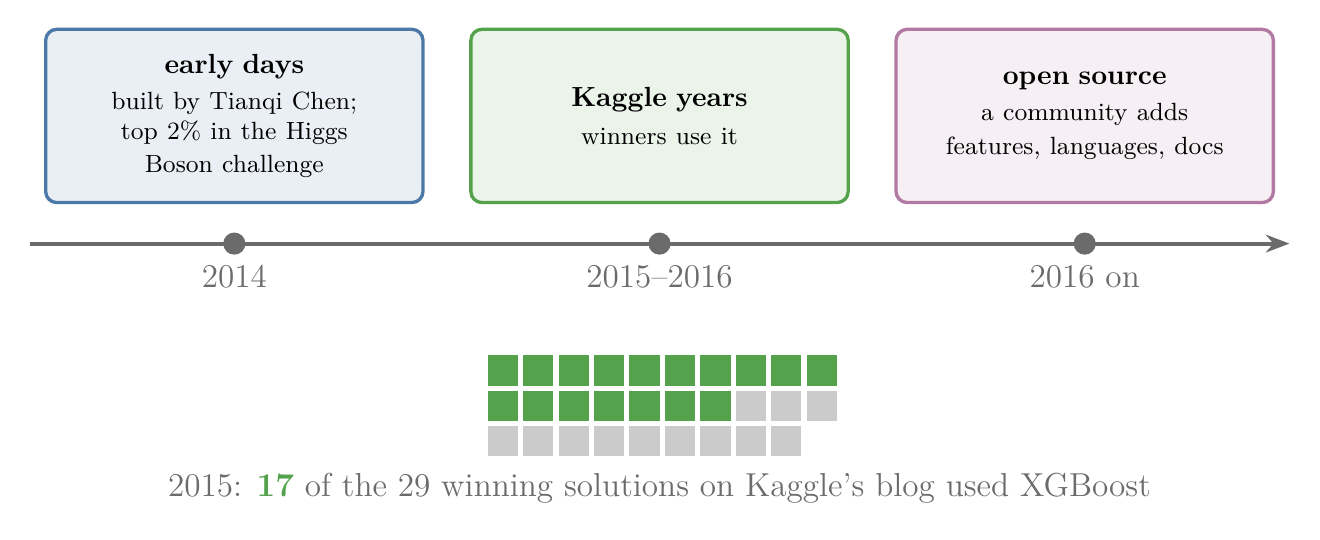
\begin{tikzpicture}[s/.style={box=#1, minimum width=4.6cm, text width=4.3cm, align=center, minimum height=2.2cm}]
  \draw[arrow] (-2.6,0) -- (13.4,0);
  \foreach \x/\yr in {0/2014, 5.4/2015--2016, 10.8/2016 on} {\fill[cgrey] (\x,0) circle (4pt); \node[note, below] at (\x,-0.15) {\large\yr};}
  \node[s=cblue, anchor=south] at (0,0.5) {\textbf{early days}\\[2pt]\small built by Tianqi Chen;\\top 2\% in the Higgs\\Boson challenge};
  \node[s=cgreen, anchor=south] at (5.4,0.5) {\textbf{Kaggle years}\\[2pt]\small winners use it};
  \node[s=cpurple, anchor=south] at (10.8,0.5) {\textbf{open source}\\[2pt]\small a community adds\\features, languages, docs};
  % 29 winning solutions of 2015, 17 with XGBoost
  \foreach \i in {0,...,28} {
    \pgfmathtruncatemacro{\c}{mod(\i,10)} \pgfmathtruncatemacro{\r}{div(\i,10)}
    \pgfmathsetmacro{\col}{\i<17 ? 1 : 0}
    \ifnum\i<17 \fill[cgreen, draw=white, line width=1pt] (3.2+0.45*\c,-1.4-0.45*\r) rectangle ++(0.42,-0.42);
    \else \fill[cgrey!35, draw=white, line width=1pt] (3.2+0.45*\c,-1.4-0.45*\r) rectangle ++(0.42,-0.42); \fi
  }
  \node[note, align=center] at (5.4,-3.1) {\large 2015: \textcolor{cgreen}{\textbf{17}} of the 29 winning solutions on Kaggle's blog used XGBoost};
\end{tikzpicture}
\end{document}
